\section{Neural networks}

Neural Networks (NNs) are computational models composed of layers of neurons that can learn from data. They are versatile and robust models capable of learning directly from raw data, without the need for manually selected features. NNs employ a training algorithm known as backpropagation, which adjusts the model's parameters based on a loss function.

\subsection{Feedforward networks}

A feedforward neural network is characterized by its architecture, devoid of cycles, where the output of layer \(i\) can be computed using the outputs from layer \(i - 1\). The architecture of a neural network encompasses its structure, including the number of hidden layers and neurons, as well as the functions employed for computations. These selections, known as hyperparameters, are parameters whose values are not determined by the learning algorithm. Figure \ref{fig:ffn} shows a typical feedforward network architecture.


\begin{figure}[H]
    \centering
    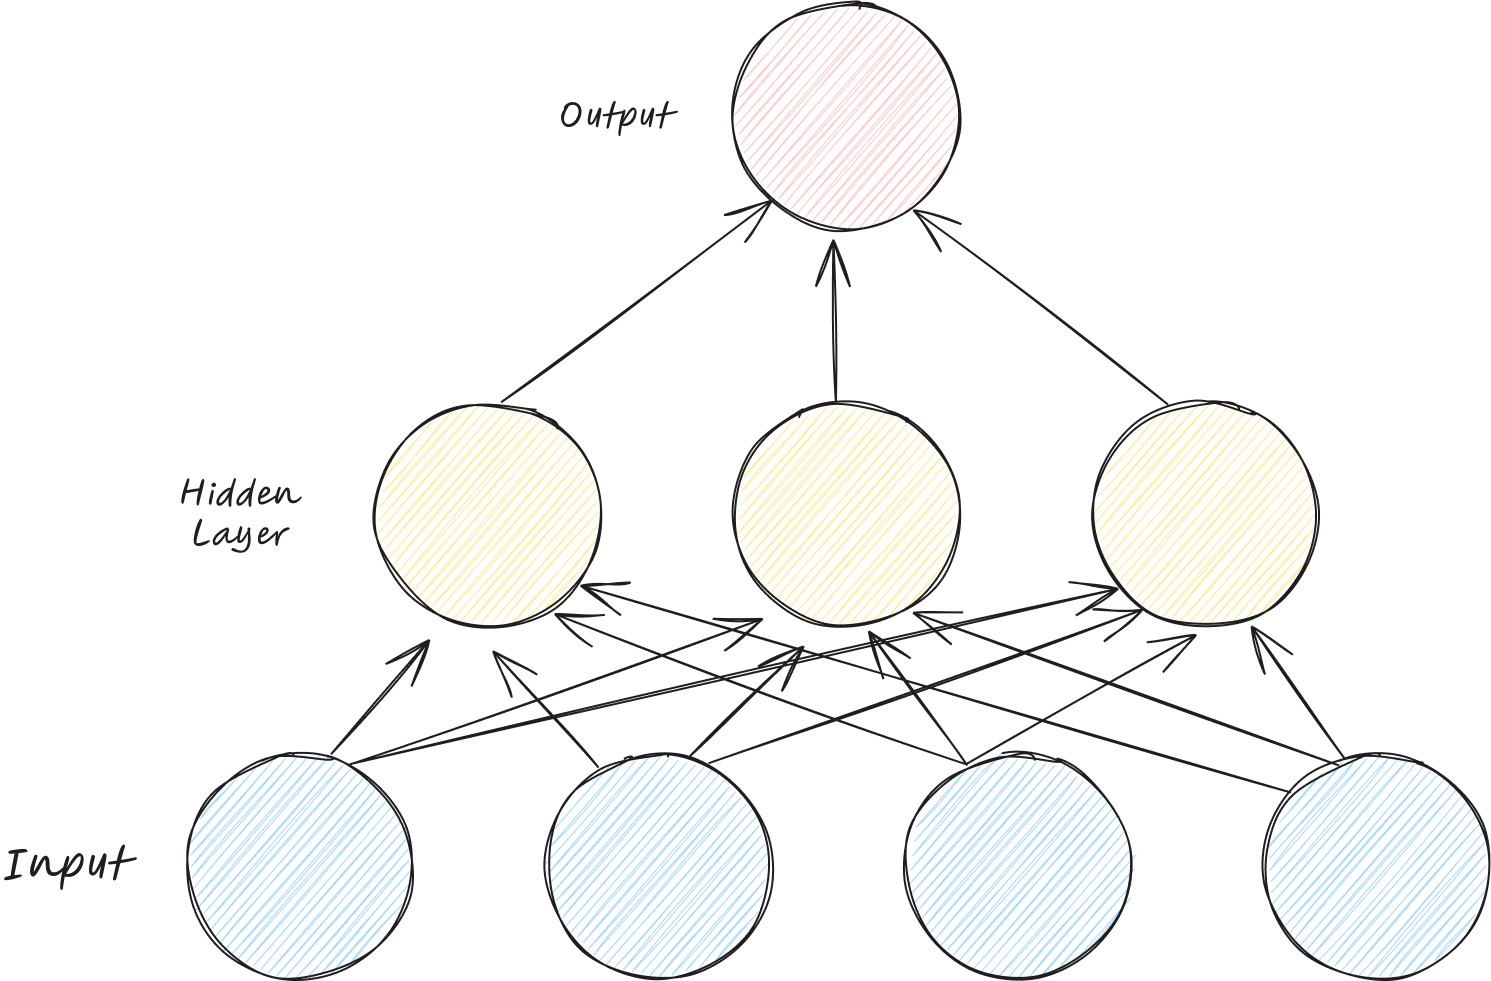
\includegraphics[width=\textwidth,height=6cm,keepaspectratio=true]{ffn.png}
    \caption{
        \it{Example of a feedforward neural network architecture. The network has an
            input layer with four neurons, one hidden layer with three neurons and an output layer with a single neuron.}
    }
    \label{fig:ffn}
\end{figure}

As depicted in Figure \ref{fig:ffn}, neural networks comprise an input layer, \(n\) hidden layers, and an output layer. The input layer receives the data that the network needs to process, which then traverses through the hidden layers before reaching the output layer. The output layer provides the model's result for the given input data. When a neural network contains multiple hidden layers, it qualifies as a deep neural network (DNN) and falls within the domain of deep learning \cite{oshea2015introduction}. Each layer consists of \(i\) neurons, with connections between each neuron in a layer and every neuron in the previous layer, except for the input layer.

Neurons serve as fundamental computational units and, as previously indicated, establish connections with all neurons in the preceding layer. Each connection is characterized by a numerical parameter referred to as a weight.


\begin{figure}[H]
    \centering
    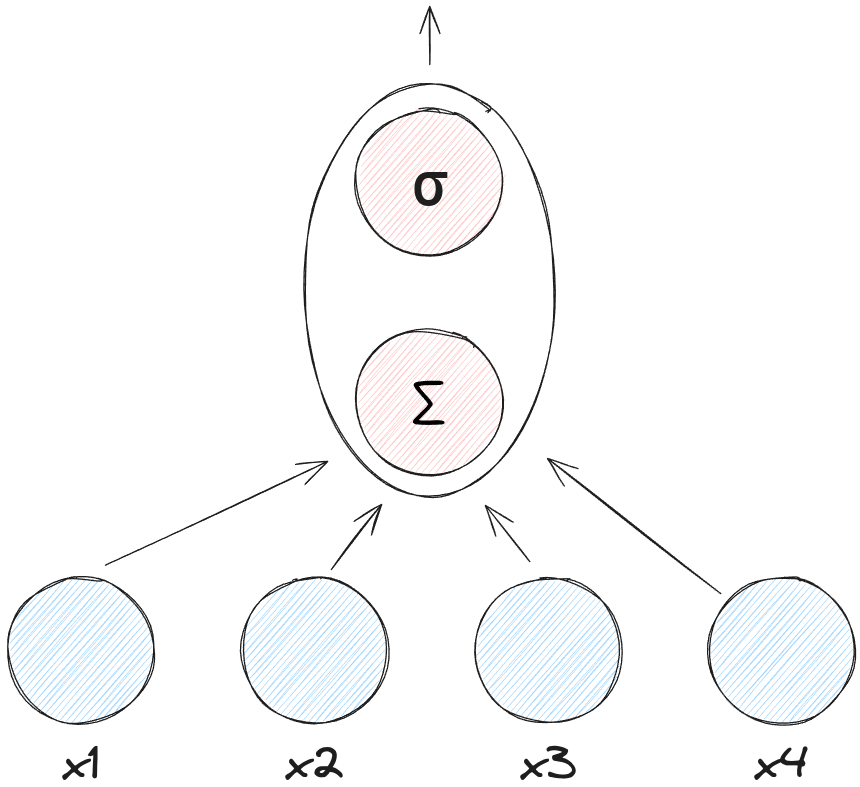
\includegraphics[width=\textwidth,height=6cm,keepaspectratio=true]{1nn.png}
    \caption{
        \it{Example of computation within a single neuron, where the weighted sum
            of inputs is passed through an activation function to get the output of the neuron.}
    }
    \label{fig:1nn}
\end{figure}

As show in Figure \ref{fig:1nn}, the neuron receives inputs from neurons of the preceding layer, denoted as \(x_1, x_2, ..., x_n\). Each neuron-to-neuron connection is assigned a weight, representing the strength of the connection. The output from a preceding neuron is multiplied by the weight of the connection and then summed for each connected neuron, yielding the weighted sum of values.

Although not visually represented in Figure \ref{fig:1nn}, a bias parameter is introduced to the weighted sum, thereby altering \(a_j\) to

\begin{equation}
    a_j = \sum_{j'} w_{jj'}x_{j'} + b
\end{equation}

The bias serves to adjust the neuron's output independently of the input. This capability enables the model to alter the neuron's output during the learning process without necessitating adjustments to the weights, thereby facilitating finer control.

The weighted sum is subsequently forwarded to an activation function, which determines the neuron's output or its degree of "activation." An illustration of such an activation function is the sigmoid function denoted as \(\sigma\), as depicted in Figure \ref{fig:1nn}. The mathematical expression for the sigmoid function is:

\begin{equation}
    \sigma(a_j) = \frac{1}{1+e^{-a_j}}
\end{equation}

According to Nielsen [19], two other common activation functions include \(\tanh \phi\),
which is defined as

\begin{equation}
    \phi(a_j) = \tanh(a_j) = \frac{e^{a_j} - e^{-a_j}}{e^{a_j} + e^{-a_j}}
\end{equation}

and Rectified Linear Unit (ReLU), which is defined by equation

\begin{equation}
    R(a_j) = max(0, a_j)
\end{equation}

Symbol \(a_j\) refers to the result of adding together the weighted sum and bias. The
outputs of these functions are visualized in Figure \ref{fig:activation}.


\begin{figure}[H]
    \centering
    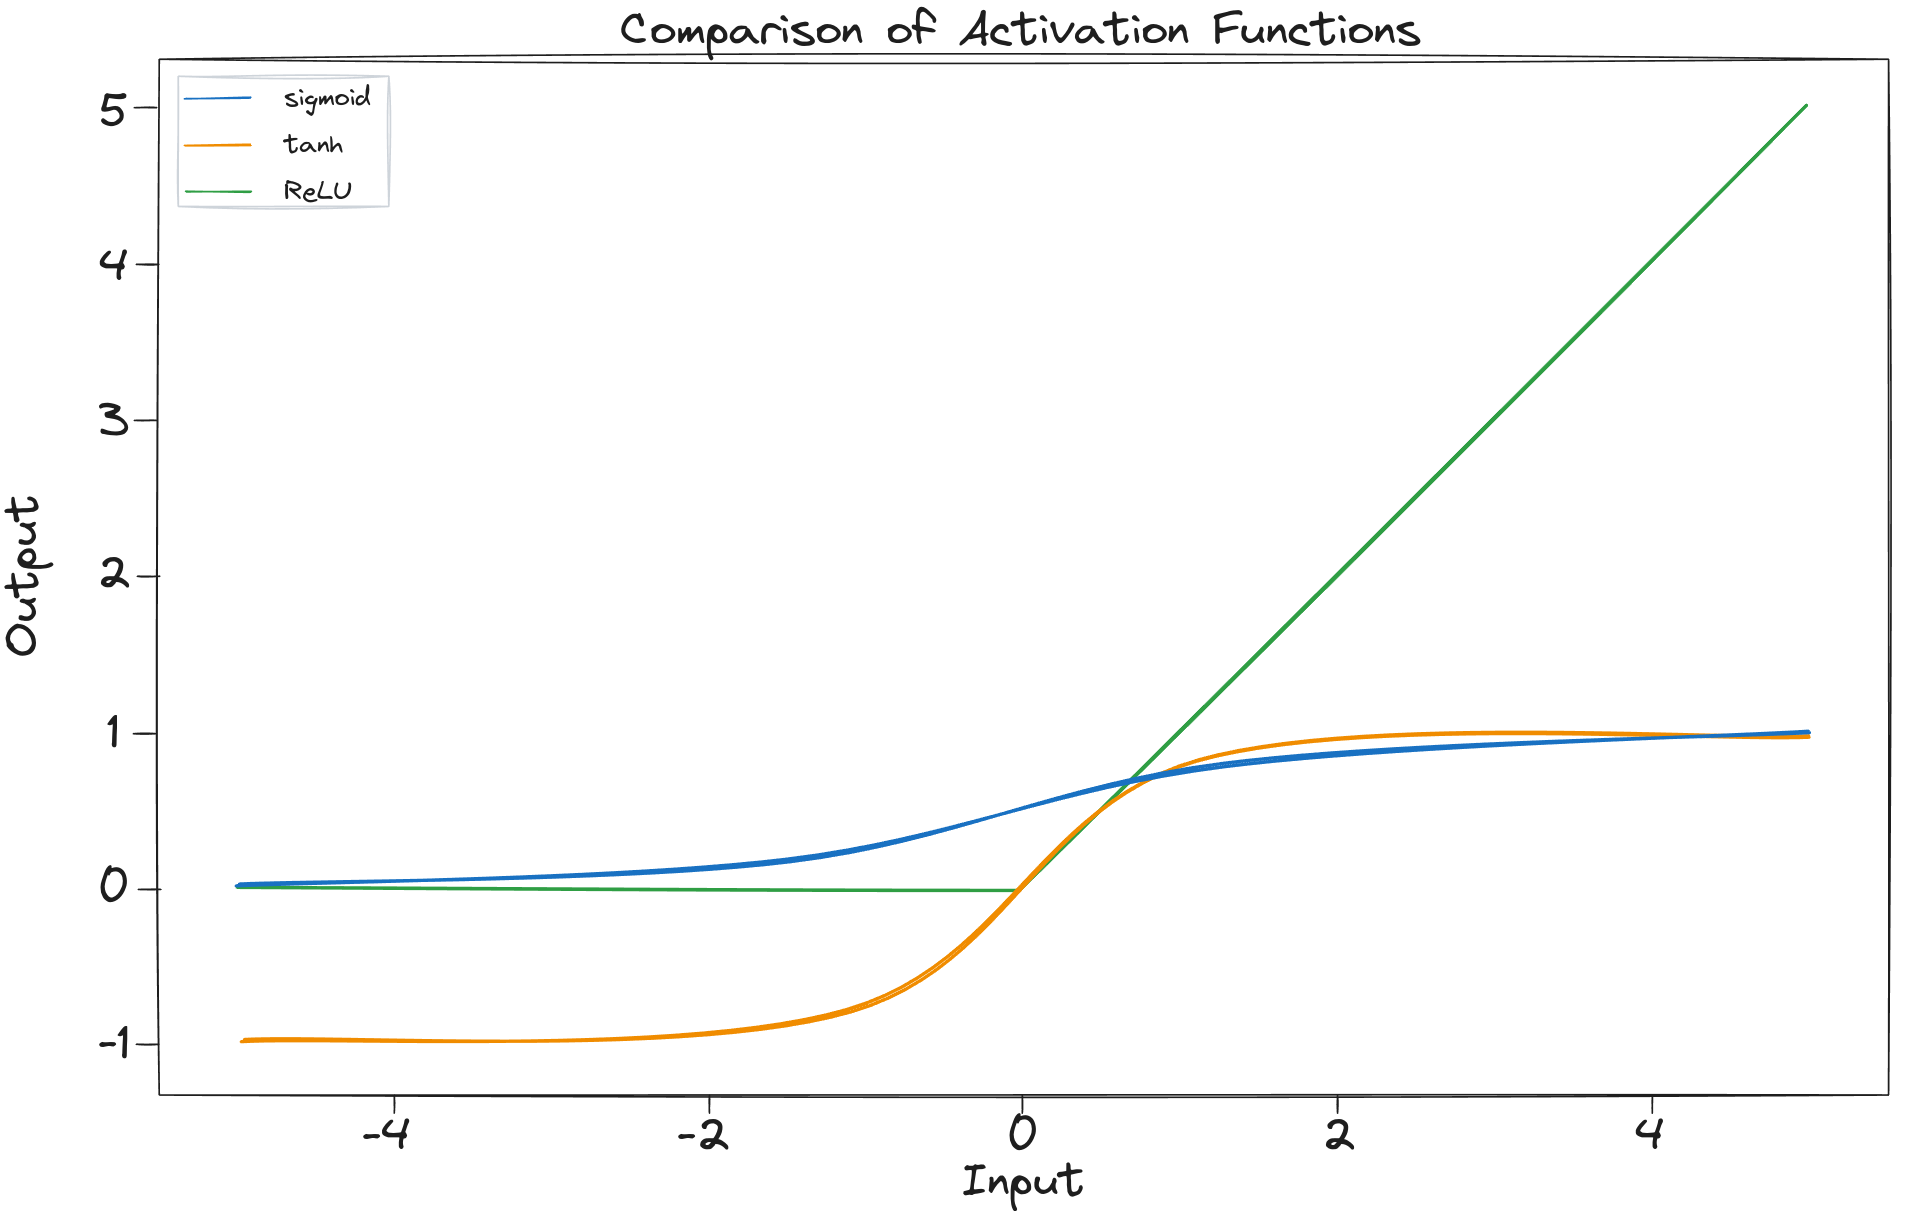
\includegraphics[width=\textwidth,height=6cm,keepaspectratio=true]{activation.png}
    \caption{
        \it{Visualization of the sigmoid, tanh and ReLU activation function outputs.}
    }
    \label{fig:activation}
\end{figure}

The outputs produced by these activation functions exhibit non-linearity, signifying that the input parameter does not linearly determine the output value, as evident from Figure \ref{fig:activation}. This concept holds significance in neural networks, enabling them to learn non-linear systems [20]. While several activation functions are commonly employed, ReLU has gained prominence in deep learning due to its demonstrated efficacy in enhancing the performance of numerous neural networks [18]. Typically, the same activation function is applied across all neurons, except for those in the output layer.

The choice of activation function for the output layer hinges on the specific task assigned to the neural network. In regression-based tasks, a linear activation function is employed to obtain the summed weighted output of the preceding neurons. Conversely, for classification problems involving \(k\) output neurons, a softmax function is often utilized. The softmax function is defined as:

\begin{equation}
    \hat{y} = \frac{e^{a_k}}{\sum_{j=1}^J e^{a_j}}
\end{equation}

\noindent and ensures that all neuron outputs sum to one on the output layer.

\subsection{Recurrent Neural Networks}
\label{sec:rnn}

Recurrent Neural Networks (RNNs) are specialized neural networks designed for processing sequential data. They operate by incorporating iterations that retain past states, enabling the network to leverage previous inputs as context for the current input [8]. Text serves as a prime example of sequential data, where individual words can be viewed as singular data points within the sequence. Consequently, RNNs can effectively process textual input by utilizing preceding words to predict the subsequent ones. Figure 5 provides an illustration of a basic RNN architecture.


\begin{figure}[H]
    \centering
    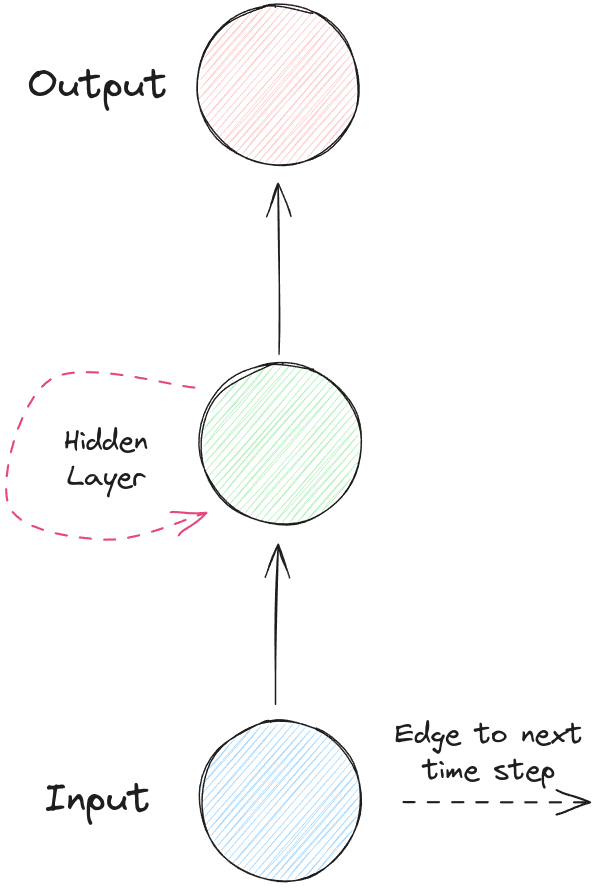
\includegraphics[width=\textwidth,height=6cm,keepaspectratio=true]{rnn.png}
    \caption{
        \it{Visualization of an RNN with one input neuron, one hidden neuron and
            one output neuron.}
    }
    \label{fig:rnn}
\end{figure}

The neuron on the hidden layer stores the hidden state, as visualized by the dashed
line. The activation of the hidden state can be defined as

\begin{equation}
    H_t = \phi_h(X_tW_{xh} + H_{t-1}W_{hh} + b_h)
\end{equation}

where \(H_t\) is the hidden state at time step \(t\), \(\phi_t\) is the activation function of the neuron, \(X_t\) is the neuron input at time step \(t\), \(W_{xh}\) is a weight matrix, \(W_{hh}\) is the weight matrix of the hidden state and \(b_h\) is bias.

RNNs are trained utilizing the backpropagation through time (BPTT) algorithm, which is an adaptation of the standard backpropagation algorithm tailored for networks with a sequential order of computations. In this setup, the output at time step \(t\) depends on the states from preceding steps [21]. During training, the forward pass computes through all time steps, and the resultant loss is utilized to update the parameters across all time steps. One way to conceptualize this process is by envisioning an unrolled RNN, where the recurrent loops are eliminated, resulting in a network structure akin to a feedforward neural network. However, due to the nature of the hidden state dynamics, RNNs are notorious for encountering gradient-related issues during training. As illustrated in Figure \ref{fig:gradient}, if the weight associated with the dotted line is less than one, future values may decrease exponentially [18]. Conversely, weights that start to grow can lead to the exploding gradient problem [8]. When gradients become too small or too large, it can impede the training process of the model.


\begin{figure}[H]
    \centering
    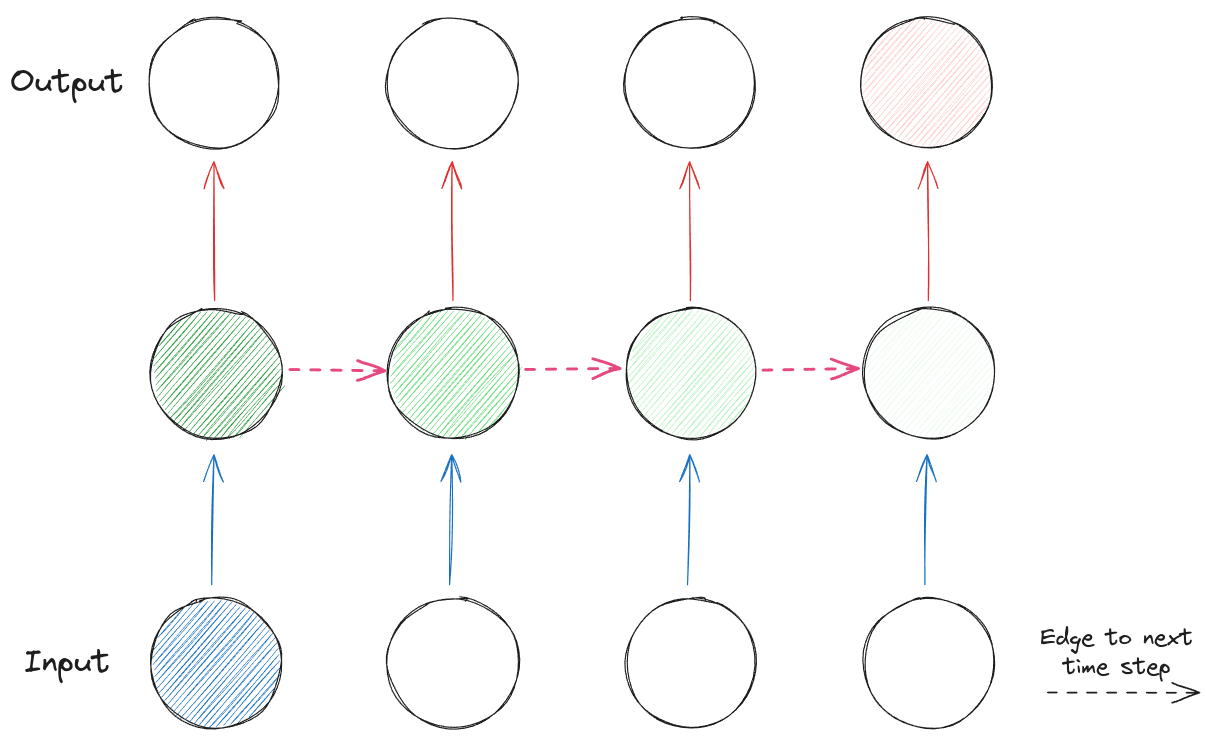
\includegraphics[width=\textwidth,height=6cm,keepaspectratio=true]{gradient.png}
    \caption{
        \it{Visualization of the vanishing gradient problem, which is indicated by the
            hidden neuron color fading away.}
    }
    \label{fig:gradient}
\end{figure}

Despite offering a robust framework for sequential learning, RNNs are hindered by significant limitations arising from the aforementioned issues. One critical limitation stems from the gradient problem encountered during training, which can constrain the effective handling of lengthy sequences. Consequently, RNNs may struggle to capture dependencies between inputs across extended sequences. To address these challenges, numerous techniques and alternative architectures have been proposed. Among these, the Long Short-Term Memory (LSTM) architecture stands out as one of the most prominent examples, and its discussion follows.

\subsection{Long Short-Term Memory}

The Long Short-Term Memory (LSTM) [9] architecture addresses the gradient-related challenges inherent in RNNs by incorporating constant error, memory cells, and gate units. This design enables the network to effectively handle sequences spanning over 1000 time steps. The memory cells employ three gate units: an input gate \(I_t\), an output gate \(O_t\), and a forget gate \(F_t\), which regulate the flow of information. Specifically, the input gate facilitates the addition of information to the memory cell, the output gate facilitates information retrieval from the cell, and the forget gate facilitates cell resetting [8]. Moreover, the memory cells possess an internal state with a self-connected recurrent edge featuring a constant weight, ensuring consistent error propagation across time steps and mitigating previously discussed gradient-related issues [18]. Additionally, a candidate memory cell \(\tilde{C}\), utilized for proposing new information, is integrated with the old memory content \(C_{t-1}\) through the gates to govern the preservation of old memory in the new memory \(C_t\) [8]. Figure 7 illustrates the complete architecture of the LSTM memory cell.

\begin{figure}[H]
    \centering
    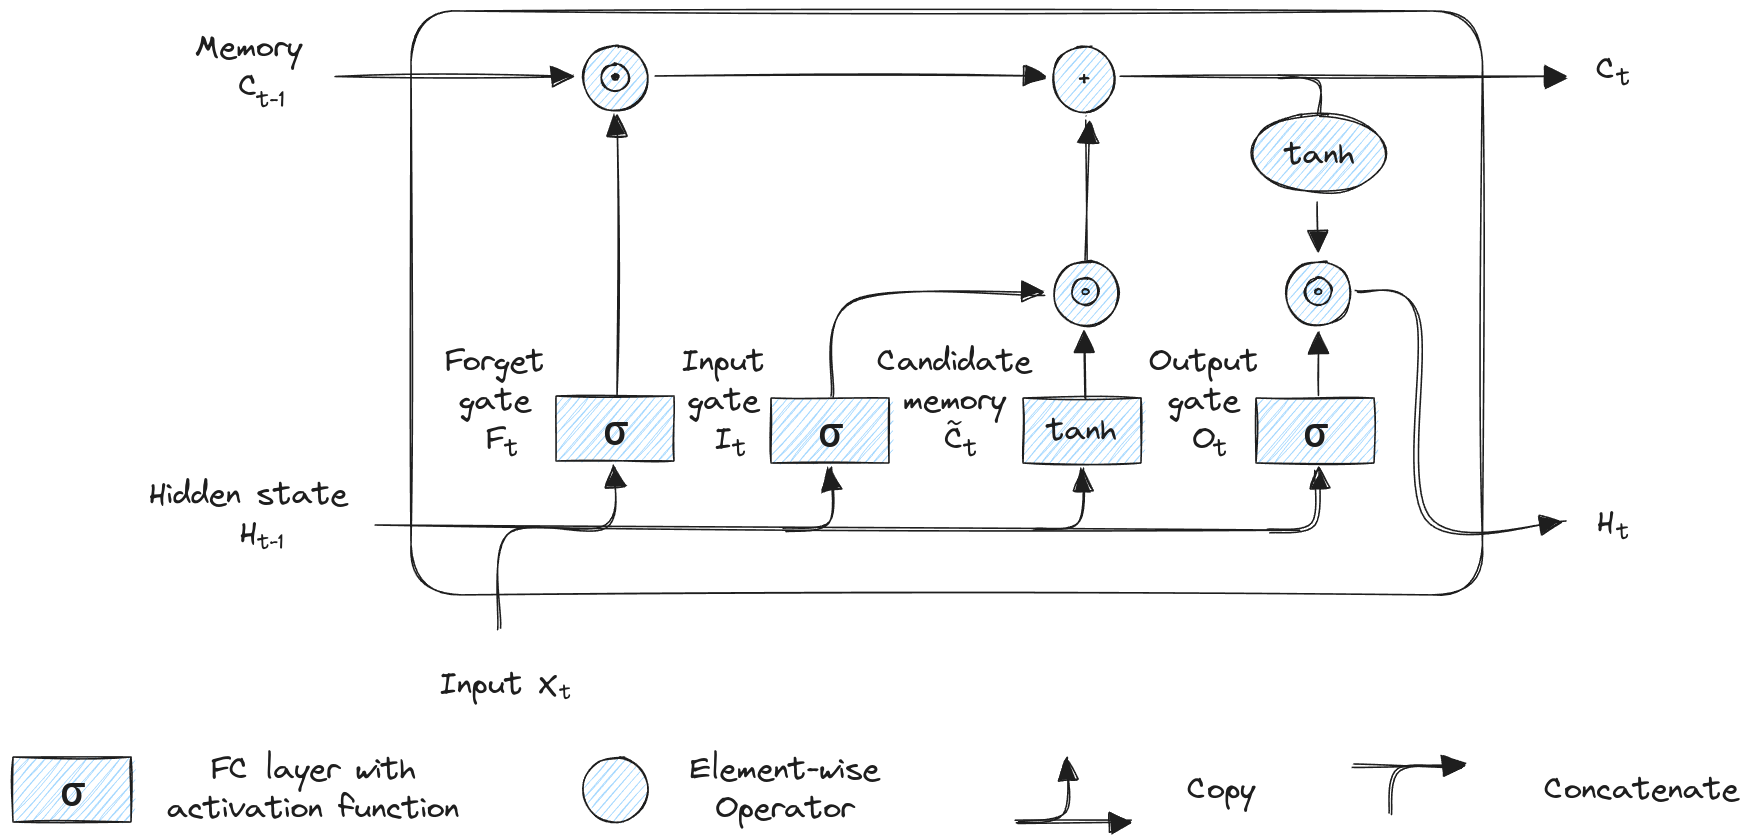
\includegraphics[width=\textwidth,height=6cm,keepaspectratio=true]{lstm.png}
    \caption{
        \it{Visualization of an LSTM memory cell.}
    }
    \label{fig:lstm}
\end{figure}

Although the LSTM architecture enhances performance compared to the RNN architecture discussed in \autoref{sec:rnn}, it still possesses limitations. Like the RNN architecture, models utilizing LSTM must process the previous time step before computing the next, rendering them computationally intensive and impeding parallelization. Additionally, LSTM typically lacks an explicit attention mechanism and tends to prioritize the most recent words. These constraints are addressed by the Transformer model, which will be introduced next.
